\chapter{Development of a Web-Based Visualization Tool for the Comparison of Organism Genome Properties} \label{micromeda-client}

As discussed in Chapter \ref{micromeda-server}, Micromeda's web visualizations interface consists of a web client backed by a separate server process. This server provides a series of web API endpoints (Section \ref{endpoints}) from which the client can acquire data about the genome properties possessed by multiple organisms. The role of the client is to visualize this data and provide a user interface for exploring it. The client is capable of visualizing data from uploaded Micromeda files. As discussed in Section \ref{MicromedaFiles}, these file contain not only property and step assignments for multiple organisms but also the protein sequences and domain annotations used to make these assignments. The client provides a way to upload these files to the server in addition to its visualization capability. In this chapter we will discuss the client web application in detail. This client is called called Micromeda-Client.

\section{Visualization Design}

\subsection{An Overview of Genome Properties Data}

The data to be presented by Micromeda-Client consists of two types: assignment data and property hierarchy data. Both of these datasets differ in their basal data types and are discussed individually below. Future versions of the Micromeda-Client may also add a third data type, InterProScan domain annotation E-value scores, as discussed in Section \ref{client-improvements}.

\subsubsection{Property Hierarchy Data}

Individual genome properties are linked together through parent-child relationships \cite{richardson2018genome}. Such relationships are hierarchical in nature. In addition, step are children of properties, adding another layer of hierarchical data. Both of these data are provided to the Micromeda-Client, via Micromeda-Server, from a \textbf{genomeProperties.txt} file (see Subsection \ref{Genome-Properties-Files}) containing a release of the Genome Properties database.

\subsubsection{Assignment Data}

Micromeda-Client, through Micromeda-Server, has access to both the assignments of support for both genome properties and property steps across multiple organisms. Such assignments provided by user uploaded Micromeda files (Section \ref{MicromedaFiles}). Such assignments are ordinal data \cite{richardson2018genome,agresti2010analysis}, as assignments YES, PARTIAL and NO are ordered. An assignment of YES lends more support than an assignment of PARTIAL and an assignment of PARTIAL lends more support than an assignment of NO. Together such assignments provide informations about the presence and absence of genome properties across organisms. It should also be noted that, due to hierarchical nature of genome properties, the assignments of parent genome properties can be used to summarize the assignments of child genome properties or property steps.

\subsection{The Use Cases for the Genome Properties Visualization}

When properties and step assignments are compared across organisms, a variety of biological insights can be derived. These comparisons can be done rapidly when such assignments are visualized. Some prominent comparisons are listed below.

\begin{itemize}
\item Looking at the assignments of a single property across organisms can be used to used for the selection of subsets of organisms which may posses a specific phenotype (Fig. \ref{fig:client-analysis-types}a). In the field of genetic engineering, such comparisons could be used for host or gene donor selection.
\item Comparing the assignments of multiple properties could be used for identifying patterns of property conservation across organisms in a dataset (Fig. \ref{fig:client-analysis-types}c). In microbial ecology, such comparisons could be used to identify microorganisms which fit specific ecological niches.
\item Looking at the steps assignments of a single property in a single organism could be used to evaluate the correctness of the property's assignment in this organism  (Fig. \ref{fig:client-analysis-types}b). For example, a property might be assigned NO or PARTIAL because it is only missing a few required step assignments but possess many others (Fig. \ref{fig:client-analysis-types}b). Being able to look at all step assignments for the property may be useful for why a property has been given an assignment.
\item Comparing the step assignments of single property across organisms can be used to see what pathway steps are retained across organisms that differ photogenically (Fig. \ref{fig:client-analysis-types}d). For example, if a property step is not retained in a large assortment of genomes, it may not be required or is carried out by proteins which are non-canonical (Fig. \ref{fig:client-analysis-types}d). Such proteins may not posses domains used by Genome Properties but may still carry out the pathways step.
\end{itemize}

\begin{figure}[!ht]
  \centering
	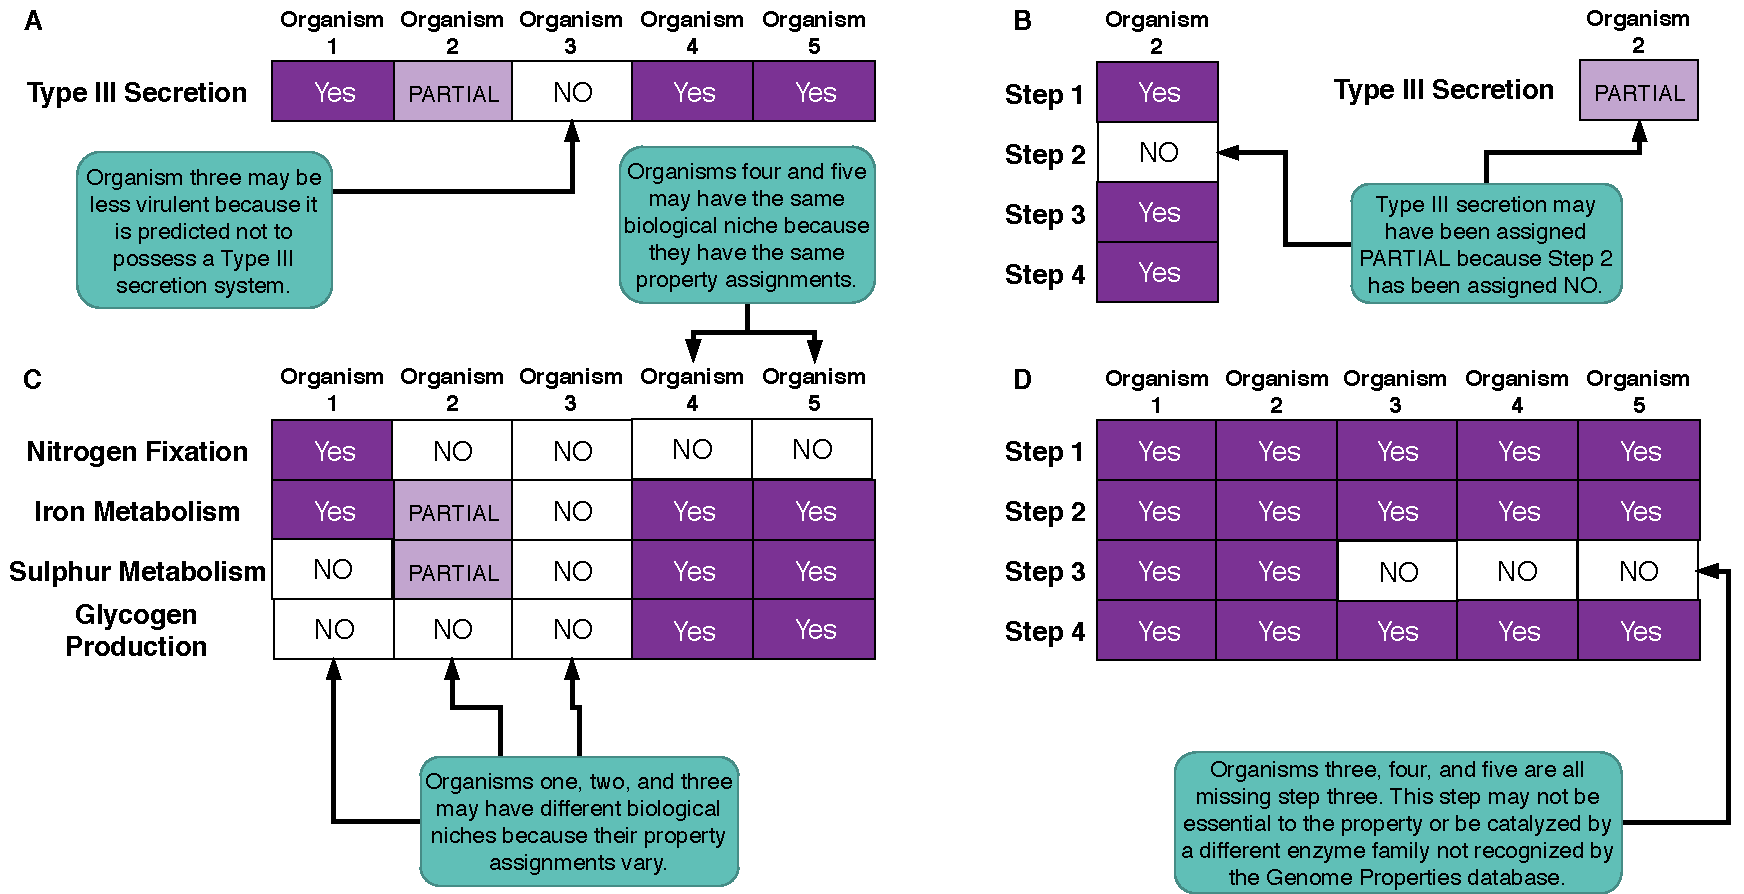
\includegraphics[width=\textwidth]{media/analysis_types.pdf}
	 \caption{Visualizations of Genome Properties data can be used to compare property and step assignments across organisms.}
	 \label{fig:client-analysis-types}
\end{figure}

\subsection{How Should Genome Properties Data Be Visualized?}

To support the above use cases Micromeda-Client's visualization components must be able to allow perform operations below.

\begin{itemize}
\item Allow users to track assignments across organisms.
\item Allow users assess the magnitude of given assignments.
\item Allow users to aggregate step and property assignments into summaries.
\item Allow users to explore how these aggregate assignments are derived.
\item Allow users to quickly find assignments of interest.
\end{itemize}

A very apt visualization for Genome Properties assignments is a heat map (Fig. \ref{fig:client-analysis-types}). In such a visualization, cell position is used to indicate what assignment belongs to which property or step and which organism in a dataset. The magnitude of each assignment is encoded using color. Since assignments are ordinal data it makes sense to encode assignments using colour saturation, rather than hue. For Micromeda-Client we chose to use such a heat map. A heat map was chosen over competing visualization techniques such as bubble plots, circular maps or tree maps due to the number of variables in and nature of the data that needed to be plotted and the superior space utilization that heat maps have. Hear maps have superior space utilisation as compared to circular plots since the mimic the square dimensions of the computer monitors they are displayed on.

When using The Genome Properties database is very large database and consists of 1296 properties and 6525 steps.

\section{Delivery Methodology}

\section{Implementation}

\section{End-User Testing}

\section{Interface Performance}

\section{Deployment}

\section{Future Improvements} \label{client-improvements}

\section{Summary} 